%% SECTION HEADER /////////////////////////////////////////////////////////////////////////////////////
\section{Sample configuration}
\label{sec:sample}

%% SECTION CONTENT ////////////////////////////////////////////////////////////////////////////////////
The sample of interest was a \numproduct{500 x 500 x 1.5} \unit{\cubic\mm} unidirectional \ac{cfrp} plate with stack sequence \(\left[\ang{0},\,\ang{90}\right]_s\) bonded to an aluminium honeycomb core.
The volume fraction of fibres was assumed 47\%.
It was decided to use only one skin, as it is pictured in Figure~\ref{fig:honeycomb}(\textbf{b}), with the intention of experimental validation and to be able to enlarge disbonds between the skin and the core located in the middle of \ac{hsc} with a tool in a real sample. 
However, separate samples were not dedicated for each size of damage because too many factors would affect the signal value, including skin and sensors properties, the thickness of the adhesive layers, position of the core relative to the sensors, and distance between sensor.
Moreover, it renders closely the realistic scenario of monitoring the same structure.
\begin{figure}[H]
	\begin{center}
		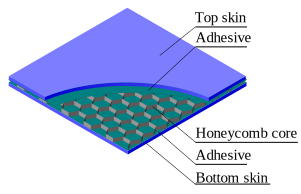
\includegraphics[width=0.95\textwidth]{Chapter_5/honeycomb}
	\end{center}
	\caption{Sample configuration: (\textbf{a}) top view of the sample, (\textbf{b}) \acl{hsc} and (\textbf{c}) details of the honeycomb cell}
	\label{fig:honeycomb}
\end{figure}

The core geometry is accurately reproduced from the actual specimen, i.e., geometry of irregular hexagonal cells \(\left(\mathrm{h}_1 \ne \mathrm{l}_1\right)\) and double walls at the sheet joints, resulting from the core fabrication technology.
According to the drawing in Figure \ref{fig:honeycomb}(\textbf{c}), the cell dimensions are \(\mathrm{w}_c=0.1\) \unit{\mm}, h\(_1\)=11 \unit{\mm}, h\(_2\)=5 \unit{\mm}, l\(_1\)=10.4 \unit{\mm}, l\(_2\)=6 \unit{\mm} and the cell height g=14.5 \unit{\mm}.
The core was bonded to one \ac{cfrp} plate using the epoxy adhesive (Loctite EA3479B) with the thickness h\(_a\)=0.3 \unit{\mm}.
The adhesive layer covered the entire bottom surface of the skin.
\nomtypeR[w_core]{\(\mathrm{w}_c\)}{Thickness of a core wall}{}{\unit{\metre}}%
\nomtypeR[h_core]{h\(_1\), h\(_2\)}{Lengths of a core cell}{}{\unit{\metre}}%
\nomtypeR[l_core]{l\(_1\), l\(_2\)}{Widths of a core cell}{}{\unit{\metre}}%
\nomtypeR[g_core]{g}{Height of a cell}{}{\unit{\metre}}%
\nomtypeR[h_adh]{h\(_a\)}{Thickness of an adhesive layer}{}{\unit{\metre}}%
\nomtypeR[h_pzt]{h\(_{PZT}\)}{Thickness of a transducer}{}{\unit{\metre}}%
\nomtypeG[phi_pzt]{\(\Phi_{PZT}\)}{Diameter of a transducer}{}{\unit{\metre}}%
\nomtypeR[h_glue]{h\(_g\)}{Thickness of a cyanoacrylate glue}{}{\unit{\metre}}%
Signal excitation and recording were accomplished with a pair of \acp{pzt}  (Noliac, NCE51) mounted to the top surface of the skin with cyanoacrylate glue.
The circular transducers of diameter \(\Phi_{PZT}\)=10 \unit{\mm} and thickness h\(_{PZT}\)=0.5 \unit{\mm} were attached 200 \unit{\mm} apart, as shown in Figure~\ref{fig:honeycomb}(\textbf{a}).
The thickness of cyanoacrylate glue under the \ac{pzt} was assumed to be h\(_g=50\) \unit{\micro\m}.

The material properties of the components assumed for the simulations are compiled in Table~\ref{tab:properties}.
The effective properties of the \ac{cfrp} skin were determined according to the rule of mixtures presented in the book by Vinson and Sierakowski \cite{vinson1993behavior}.
The authors provide a complete description of the homogenisation of composite properties.
Firstly, the stiffness matrix was determined for the single ply of the laminate along the fibre direction.
Then, the stiffness matrix was transformed for other orientations of the laminate plies by the transformation matrix composed of the direction cosines.
In the analysed sample, there were plies with an orientation of \ang{0} and \ang{90}.
Finally, all the plies in the laminate were homogenised through the thickness.
Sun and Li \cite{sun1988three} present the explicit expressions of the stiffness components for the laminate modelled by solid elements.
The comprehensive equations to derive the effective stiffness matrix are given in Appendix~\ref{app:eff_properties}, whereas Table~\ref{tab:properties_eff} shows the resulting \ac{cfrp} properties.
\begin{table}[H]
	\centering
	\small
	\tabcolsep=0.25cm
	\caption{\label{tab:properties_eff} The homogenised mechanical properties of the \acs{cfrp} plate and the honeycomb core for +20\unit{\degreeCelsius}}
	\begin{tabular}{ccccccccc}
		\toprule
		\multirow{2}{*}{\textbf{Material}} & \(\boldsymbol{E_{11}}\) & \(\boldsymbol{E_{22}}\) & \(\boldsymbol{E_{33}}\) & \(\boldsymbol{G_{12}}\) & \(\boldsymbol{G_{23}}\) & \(\boldsymbol{\nu_{12}}\)	& \(\boldsymbol{\nu_{23}}\) & \(\boldsymbol{\rho}\) \\
		& \unit{\giga\pascal} & \unit{\giga\pascal} & \unit{\giga\pascal} & \unit{\giga\pascal} & \unit{\giga\pascal} & -- & -- & \unit[per-mode = symbol]
		{\kilogram\per\cubic\metre}\\
		\midrule
		\ac{cfrp} & 69.5 & 69.5 & 8.16 & 3.43 & 2.96 & 0.03 & 0.37 & 1555\\
		laminate & & & & & & & &\\
		\midrule
		honeycomb & 0.007 & 0.005 & 2.76 & 0.002 & 0.86 & 0.999 & \(\approx0\) & 112\\
		core & & & & & & & &\\
		\bottomrule
	\end{tabular}
\end{table}
\nomtypeR[G]{\(G\)}{Shear modulus}{}{\unit{\giga\pascal}}%